\documentclass[10pt]{llncs}

%\usepackage{doc}
%\usepackage{makeidx}
\usepackage{fancyvrb}
\usepackage{listings}
\usepackage{longtable}
\usepackage{paralist}
\usepackage{color}
\usepackage{algpseudocode}
\usepackage{hyperref}
\usepackage{graphicx}
\usepackage{mathtools}
\usepackage{amsfonts}
\usepackage{stmaryrd}
\usepackage{amsmath}
\usepackage{verbatim}
\usepackage{txfonts}
\hypersetup{
    colorlinks,
    citecolor=black,
    filecolor=blue,
    linkcolor=black,
    urlcolor=blue
}
% for overriding caption view
\usepackage{caption}
\captionsetup[lstlisting]{ singlelinecheck=false, margin=0pt, font={it,footnotesize} }

% Let's style the code!
% Set-up code visualisation
\lstset{fancyvrb=true}
\lstset{
language=java,                  % the language of the code
basicstyle=\footnotesize,       % the size of the fonts that are used for the code
numbers=left,                   % where to put the line-numbers
numberstyle=\footnotesize,      % the size of the fonts that are used for the line-numbers
stepnumber=1,                   % the step between two line-numbers. If it's 1, each line 
                                % will be numbered
numbersep=5pt,                  % how far the line-numbers are from the code
keywordstyle=\color{blue},
commentstyle=\color{green},
stringstyle=\color{red},
backgroundcolor=\color{white},  % choose the background color. You must add \usepackage{color}
showspaces=false,               % show spaces adding particular underscores
showstringspaces=false,         % underline spaces within strings
showtabs=false,                 % show tabs within strings adding particular underscores
frame=single,                   % adds a frame around the code
tabsize=2,                      % sets default tabsize to 2 spaces
captionpos=t,                   % sets the caption-position to bottom
breaklines=true,                % sets automatic line breaking
breakatwhitespace=false,        % sets if automatic breaks should only happen at whitespace
%title=\lstname,                 % show the filename of files included with \lstinputlisting;
                                % also try caption instead of title
escapeinside={\%*}{*)},         % if you want to add a comment within your code
morekeywords={*,...}            % if you want to add more keywords to the set
}
\lstset {
    keywordstyle=\color[rgb]{0,0,1},          % keywords in blue
    commentstyle=\mcommentfont,               % comments
    stringstyle=\color[rgb]{.627,.126,.941},  % strings in purple
    commentstyle=\color[rgb]{.133,.545,.133}
}

% In order to save space or manage large tables or figures in a
% landcape-like text, you can use the rotating and pdflscape
% packages. Uncomment the desired from the below.
%
% \usepackage{rotating}
% \usepackage{pdflscape}

% If you plan on including some algorithm specification, we recommend
% the below package. Read more details on the custom options of the
% package documentation.
%
% \usepackage{algorithm2e}

%\makeindex

%% Document
%%


% Regular title as in the article class.
\title{Ensuring Faultless Communication Behaviour\\
       in a Commercial Cloud Application}

% \titlerunning{} has to be set to either the main title or its shorter
% version for the running heads.
\titlerunning{Faultless Communication in a Cloud}

% Authors are joined by \and. Their affiliations are given by \inst, which indexes
% into the list defined using \institute
\author{
	Ross Horne, Rustem A. Kamun \and Timur Umarov
}

% Institutes for affiliations are also joined by \and,
\institute{
  Faculty of Information Technology, Kazakh-British Technical University, 
  Almaty, Kazakhstan
  \email{ross.horne@gmail.com \quad r.kamun@gmail.com \quad t.umarov@kbtu.kz}
}

%  \authorrunning{} has to be set for the shorter version of the authors' names.
\authorrunning{R. Horne, R. Kamun \& T. Umarov}

\begin{document}

%%%%%%%%%%%%%%%%%%%%%%%%%%%%%%%%%%%%%%%%%%%%%%%%%%%
\maketitle
%%%%%%%%%%%%%%%%%%%%%%%%%%%%%%%%%%%%%%%%%%%%%%%%%%%

\begin{abstract}
%The scale and complexity of Web Services raises the challenge of controlling their interaction.
The goal of this work is to ensure that processes that integrate several services in a Cloud correctly interact according to a specification of their communication behaviour. To accomplish this goal, we employ session types to analyse the global and local communication patterns. A session type represents a ``formal blueprint'' of how users and services should interact with the Cloud at an appropriate level of abstraction for specifying message flows.
 
This work confirms the feasibility of applying session types to business protocols used by an e-commerce Cloud provider. The protocols are developed in SessionJ, an extension of Java implementing session-based programming. Furthermore, we highlight how our approach can be used to intergrate services across multiple Cloud providers, each of whom must correctly cooperate.
\end{abstract}

\setcounter{tocdepth}{2}
%\small\tableofcontents}

\pagestyle{empty}


%------------------------------------------------------------------------------
\section{Introduction}
\label{sect:introduction}

%The growing needs for information availability and accessibility present new challenges for application development.
%The need for distributed highly available services presents challenges for application development.
%Two forces working in parallel with regards to the need for integration.
Cloud providers typically offer a portfolio of services, where access and billing for all services are integrated in a single distributed system. %made available at a single entry point of entry. %and simple billing where several services are integrated.
Services are then made available on demand to anyone with a credit card, eliminating the up front commitment of users~\cite{Armbrust2010}.
Furthermore, there is a drive for services to be integrated, not only within a Cloud, but also between multiple Cloud providers~\cite{utility-driven-fed}. %n enterprise, and between businesses.
%Web services are appropriate for integrating software applications within and across organizational boundaries.
%In this setting, each service is an independently deployed applications that interacts with processes according to a protocol.
%are then interconnected using a stack of standards. %(depicted in Figure~\ref{fig:soa-stack}). 

Protocols that integrate heterogeneous services with a single point of access and billing strategy can become complex. Thus we require an appropriate level of abstraction to specify and implement such protocols. Further to the complexity, the protocols are a critical component of the business strategy of a Cloud provider. Failure of the protocols could result in divergent behaviour that jeopardises services, leading to loss of customers or even legal disputes. These risks can be limited by using techniques that statically prove that protocols are correct and dynamically check that protocols are not violated at runtime.

It is challenging to manage service interactions that go beyond simple sequences of requests and responses or involve large numbers of participants. %(multi-party communication).
%A need arises for new transaction implementations, more suitable for the Web.
One technique for managing protocols between multiple services is to specify the protocol using a choreography.
A choreography specifies a global view of the interactions between participating services. % engage and interconnections between these interactions, including control-/data-flow dependencies.
However, by itsself, a choreography does not determine how the global view can be executed.
%However, a choreography does not describe internal effects within a participating service.

%, and, therefore, its functionality is not clear.
\begin{comment}
		\begin{figure}[ht]
		\begin{centering}
		\scalebox{0.7}{
		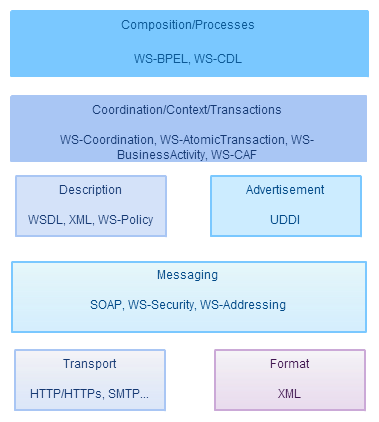
\includegraphics[width=0.5\textwidth]{resources/WS_stack.png}
                }
		\caption{Stack of WS Standards}
		\label{fig:soa-stack}
		\end{centering}
		\end{figure}
\end{comment}

%Applications include business transactions operating in closely coupled context (e.g.\ the online stock exchange (ForEX), and e-commerce services based on Buyer-Seller-Shipper (BSH) protocols).
%Highly available services are likely to have a long life span that may result in deadlock.
%Although,in closely coupled settings, the SOA standards may incur a significant performance overhead.

%In addition there is no special concept of the participants of communication. 

\begin{comment}
	\begin{compactenum}
	   \item business transactions with short life span, operating in closely coupled context, where SOA standards may become a trap (online stock exchange(ForEX), services based on BSH protocol\footnote{Buyer-Seller-Shipper protocol} such as e-commerce services);
	   \item applications with a long life span that may result in deadlock.
	\end{compactenum}
\end{comment}

%The concept of a participant in a communication is essential in complex interactions.
%Much literature exist on the specification of systems that describe services from the local perspective of a participant~\cite{cs-processes,alg-seq-processes,Milner1992}.
The challenge of controlling interactions of participants motivated the design of Web Services Choreography Description Language (WS-CDL)~\cite{session-types-sessions}.
The WS-CDL working group identified critical issues~\cite{ws-critical-overview} including:
\begin{compactenum}
	\item the need for tools to validate conformance to choreography specifications to ensure correct cooperation between Web Services;
	\item design time verification of choreographies to guarantee correctness of properties such as deadlock and livelock, as well as the conformance of the behaviour of participants.
\end{compactenum}

The aforementioned challenges can be tackled by adopting a solid foundational model, such as session types~\cite{session-types-sessions,carbone2007structured}. Successful approaches related to session types include: %the Chor programming language of Carbone and Montesi~\cite{chor-lang} based on sessions and trace sets~\cite{chor-essence};
 SessionJ~\cite{sj-lang}, Scribble~\cite{honda2011scribbling} and Session C~\cite{ng2012multiparty} due to Honda and Yoshida; Sing\#~\cite{basu2012deciding} that extends Spec\# with choreographies; and UBF(B)~\cite{armstrong2002getting} for Erlang.

In this paper, we present a case study where the interaction of process that integrate services in a commercial Cloud provider\footnote{V3na Cloud Platform. AlmaCloud Ltd., Kazakhstan. \url{http://v3na.com}} are controlled using session types. Session types ensure communication safety by verifying that session implementations of each participant (the users, the services and the Cloud), conform to the specified protocols. In our case study, we use SessionJ, an extension of Java supporting sessions, to specify protocols used by the Cloud provider that involve iteration and higher order communication.
%Session Java works by specifying the intended process transaction protocol using session types and implementing the interaction using session operations.

%Through these we are aiming to confirm the suitability of Session-Java as an implementation of business to business transactions. We want to explore the agility and robustness of the language and the scalability as scenarios vary in size but also complexity. In addition we will be looking for things such as ease of programming in SJ, any limitations, bugs or non-implementable scenarios.


In Section~\ref{sect:basics} we provide an overview of SessionJ.
In Section~\ref{sect:impl}, we explain and refine a protocol used by a Cloud provider and implemented using SessionJ. %and how they can be implemented correctly using session programming.
Finally, in Section~\ref{sect:highlights}, we suggest that session types can be used in the design of reliable inter-Cloud protocols, following the techniques employed in this work.


%------------------------------------------------------------------------------
\section{Methodology for Verifying Protocols in SessionJ}
\label{sect:basics}

We chose SessionJ for the core of our application, since Java was already used for several services. Furthermore, the language has a concise syntax and an active community.

We briefly outline how SessionJ is employed to correctly implement protocols.
%Session programming can be applied when participants cooperate according to specified protocols.
%Session types are formal specifications of protocols, that describe structured sequences of interaction including basic message passing, branching and recursion.
Firstly, the global protocol is specified using a global calculus similar to sequence diagrams. Secondly, the global calculus is projected to sessions types, which specify the protocol for each participant.
Thirdly, the session is implemented using operations on session sockets. The correctness of the global protocol can be verified by proving that the implementation of each session conforms to the corresponding session type.

%according to the protocol using Session programming begins from the protocols specification for interaction (using session types), which can then be concretely implemented using structured communication operations available on session sockets.


\begin{comment}
A session is an instance of a session type, i.e.\ the unit of interaction encapsulating one run of a protocol. From the perspective of abstraction, each session, is conducted on a separate channel. 

Session programming in SJ consists of the following ordered actions:

\begin{compactenum}
  \item design specification (protocol) of target communication;
  \item mapping protocols into the programs for each participant. For instance, in BSH protocols, we can distinguish three main participants whose actions (processes) are mapped to corresponding programs (software component);
  \item By utilizing session programming constructs, implementing the protocol, where each operation is performed as method call;
  \item verification of sessions fulfilment by  compiler;
  \item execution and system testing.
\end{compactenum}
\end{comment}


\begin{figure}
\begin{gather*}
\begin{array}{c}
L_1, L_2\quad\mbox{label}
\\[10pt]
p\quad\mbox{protocol name}
\\[10pt]
M \Coloneqq \textit{Datatype} \mid T \quad\mbox{message}
\\[10pt]
S \Coloneqq  p\left\{ T \right\} \quad \mbox{protocol}
\end{array}
\qquad
\begin{array}{rlr}
T \Coloneqq & T\mathbin{.}T & \mbox{Sequencing} \\ 
       \mid & \texttt{begin} & \mbox{Session initiation} \\
       \mid & \mathopen{!}\left<M\right> & \mbox{Message send} \\ 
       \mid & \mathopen{?}\left(M\right) & \mbox{Message receive} \\
       \mid & \left\{L_1 \colon T_1,\dots, L_n \colon T_n \right\} & \mbox{Session branching} \\ %??Why not use the ASCII syntax, since you use it in examples. was \oplus \left\{L_1 \colon T_1,\dots, L_n \colon T_n \right\}
       \mid & \left[T\right]* & \mbox{Session iteration} \\ 
       \mid & \texttt{rec}\,L\left[T\right] & \mbox{Session recursion scope} \\ 
       \mid & \mathopen{\#}L & \mbox{Recursive jump} \\ 
       \mid & \mathopen{@}p & \mbox{Protocol reference} \\
\end{array}
\end{gather*}
\caption{SessionJ protocol specification using session types ($T$).}\label{tab:prot-spec} 
\end{figure}
\begin{comment}
\begin{array}{rl}
P \Coloneqq & P; P             \\
       \mid & s.request() 	\\
       \mid & s.send(m)   	\\
       \mid & s.receive() 	\\
       \mid & s.outbranch(L) \ \{P\} \\
       \mid & s.inbranch() \ \{case L1\mathopen{:} {P1}\dots case Ln\mathopen{:}{Pn}\} \\
       \mid & s.outwhile(cond) \ \{P\} \\
       \mid & s.inwhile() \ \{P\} \\
       \mid & s.recursion(L) \ \{P\} \\
       \mid & s.recurse(L) \\
\end{array}
\end{comment}


\paragraph{Protocol Specification.}
%Session programming begins by declaring the protocol for the intended cooperation, where a name identifies the protocol.
%following the standard Java naming rules. %What are the standard Java naming rules. Can we not put these in the same figure.

The body of a protocol defines a \textit{session type}, according to the grammar in Figure~\ref{tab:prot-spec}.
The session type specifies the actions that the participant in a session should perform. In SessionJ, the behaviour of an implementation of a session is monitored by the associated protocol, as enforced by the SessionJ compiler and runtime. %(Polyglot\footnote{\url{http://www.cs.cornell.edu/Projects/polyglot/}. Extensible compile framework.}).
The constructs in Figure~\ref{tab:prot-spec} can describe a diverse range of complex interactions, including message passing, branching and iteration. Each session type construct has its dual construct, because a typical requirement is that two parties implement compatible protocols such that the specification of one party is dual to another party.



\paragraph{Higher Order Communication.}
\begin{comment}
For flexibility, SJ features subtyping.
Subtyping enhances the the type system by allowing the participants in a session to follow different protocols which are compatible 
Such communication can be expressed by the following dual constructs:
%
\begin{equation*}
\mathopen{!}\left<\mathopen{?}\left(\text{int}\right)\right> \hspace{2cm} \mathopen{?}\left(\mathopen{?}\left(\text{int}\right)\right)
\end{equation*}
\end{comment}
SessionJ allows message types to themselves be session types. This is called higher-order communication and is supported by using subtyping~\cite{higher-order-comm}.
Consider the dual constructs $\mathopen{!}\left<\mathopen{?}\left(\text{int}\right)\right>$ and $\mathopen{?}\left(\mathopen{?}\left(\text{int}\right)\right)$. 
These types specify sessions that expect to respectively send and receive a session of type $\mathopen{?}\left(\text{int}\right)$.
Higher order communication is often referred to a session delegation. Figure \ref{fig:sj-delegation} shows a basic delegation scenario.

In Figure~\ref{fig:sj-delegation}, the left diagram represents the session configuration before the delegation is performed: the user is engaged in a session $s$ of type $\mathopen{!}\left<\text{int}\right>$ with the Cloud, while the Cloud is also involved in a session $s'$ with a service of type $\mathopen{!}\left<\mathopen{?}\left(\text{int}\right)\right>$. So, instead of accepting the integer from the user, Cloud delegates his role in $s$ to the service.
%After delegation, SaaS can instead receive the message from the user. 
The diagram on the right of Figure~\ref{fig:sj-delegation} represents the session configuration after the delegation has been performed: the user now directly interacts with the service for the session $s$.
The delegation action corresponds to a higher-order send type for the session $s'$ between the Cloud and the service.
%
\begin{figure}[ht]
\centering
\scalebox{0.7}{
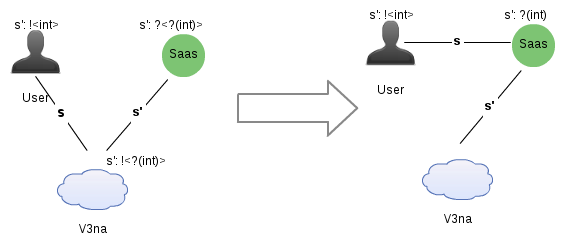
\includegraphics[width=0.8\textwidth]{resources/sj-delegation.png}}
\caption{Session delegation}\label{fig:sj-delegation}
\end{figure}

\paragraph{Protocol Implementation using SessionJ.}
%\paragraph{Another meaning for sockets}
Session sockets represent the participants of a session connection.
Each socket implements the session code according to the specified session type.
In SessionJ session sockets extend the abstract \textit{SJSocket} class. %\textit{SJRSocket::SJSocket} and \textit{SJFSocket::SJSocket}.
%Each party owns one endpoint and performs the specified interactions via the SJ session operations on that endpoint.
 %both, employ TCP as underlying transport.
%SJ distinguishes client and server sockets, where the former are used to request sessions from the latter.
%After creating a protocol (session type) and encapsulating the session into SJ socket,
The session is implemented within a session-try scope using a vocabulary of session operations. %operation  the session operations depicted in Figure \ref{tab:session-ops}.

\begin{comment}
\begin{figure}
\begin{gather*}
\begin{array}{lrl}
s.request() 	&   		    & \mbox{\texttt{begin}} \\
s.send(m)   	&  	 		& \mathopen{!}\left<M\right> \\
s.receive() 	&  	 		& \mathopen{?}\left(M\right) \\
s.outbranch(L) \ \{P\} &  		& \mathopen{!}\left\{L\mathopen{:} T\right\} \\
s.inbranch() \ \{case L1\mathopen{:} {P1}\dots case Ln\mathopen{:}{Pn}\} &   & \mathopen{?}\left\{L_1\colon 
                                        T_1,\dots, L_n\colon T_n\right\} \\
s.outwhile(cond) \ \{P\} 		&   & \left[T\right]\mathopen{*} \\
s.inwhile() \ \{P\} 		 	&   & \mathopen{?}\left[T\right]\mathopen{*} \\
s.recursion(L) \ \{P\} &   & \texttt{rec}\,L\left[T\right] \\
s.recurse(L) &   & \mathopen{\#}L \\
\end{array}
\end{gather*}
\caption{SJ protocol specification}\label{tab:session-ops} 
\end{figure}
\end{comment}

\begin{comment}
\[
\begin{array}{rlrl}
P \Coloneqq & P; P              &                                                               & T_0.T_1 \\
       \mid & s.request() 	&   		    						& \mbox{\texttt{begin}} \\
       \mid & s.send(m)   	&  	 							& \mathopen{!}\left<M\right> \\
       \mid & s.receive() 	&  	 							& \mathopen{?}\left(M\right) \\
       \mid & s.outbranch(L) \ \{P\} &  	                                        	& \mathopen{!}\left\{L\mathopen{:} T\right\} \\
       \mid & s.inbranch() \ \{case L1\mathopen{:} {P1}\dots case Ln\mathopen{:}{Pn}\} &   	& \mathopen{?}\left\{L_1\colon T_1,\dots, L_n\colon T_n\right\} \\
       \mid & s.outwhile(cond) \ \{P\} 		&						& \left[T\right]\mathopen{*} \\
       \mid & s.inwhile() \ \{P\} 		 	&   					& \mathopen{?}\left[T\right]\mathopen{*} \\
       \mid & s.recursion(L) \ \{P\} &   							& \texttt{rec}\,L\left[T\right] \\
       \mid & s.recurse(L) &              							& \mathopen{\#}L \\
\end{array}
\]
\end{comment}

%The session operations are invoked via session in a method call-like manner.
\begin{comment}
\begin{lstlisting}
s1.send(s2) // !<T>, where T is the remaining session type of 's2'
\end{lstlisting}
\end{comment}
\begin{comment}
To delegate a session, the session socket variable must be passed to a send operation on the target session.
For example, assuming that $s2$ is an active session of type $T$, then the type of $s1.\textit{send}(s2)$ is $\mathopen!\left<T\right>$.
The corresponding receive operation, $\textit{SJSocket}~s2 = s1.\textit{receive}()$ receives delegated sessions.
\end{comment}
%Only active session sockets can be delegated.

%------------------------------------------------------------------------------
\section{Case Study: Protocols for a Cloud}
\label{sect:impl}

Our case study is an e-commerce Cloud application, V3na, that provides integrated Software as a Service solutions for business. V3na provides a central access point to several services, including document storage, document flow, and customer relations management. 
The central component of the e-commerce Cloud is responsible for seamless integration and maintenance of the services that a user subscribes to, while managing user accounts and billing.

A typical scenario is when a user requires the document storage service. The user will first subscribe for the service either by registering to be billed or by entering a trial period. When the user has subscribed for the document service and they attempt to access their documents, requests to the API of the document store are delegated, by V3na, to the relevant document server for a lease period. After delegation, the client interacts directly with the API of the document store until the lease expires.

%Our case study is an e-commerce Web portal called V3na that sells SaaS applications for business needs
%V3na\footnote{\url{http://v3na.com}. Cloud platform for optimizing your business performance. Source code available at \url{https://github.com/Rustem/Master-thesis}.}
%was developed in the Django framework --- a high-level Web framework for Python. %Further information: \url{https://www.djangoproject.com/}}.
%The persistence layer is based on MongoDB and Memcached.
A major challenge was to automate the process of service integration as a reliable service.
In particular, V3na implements the following problems that can be addressed using sessions types:
%By integration, we understand the following processes with a particular SaaS application:
%
\begin{compactitem}
\item  A customer can connect to a service for a trial period; %by simply clicking on the button;

\item  V3na provides one entry point to all services a user subscribes to;

\item  A subscription may be extended or frozen;

\item  Billing and payment for use of a service can be managed.
\end{compactitem}
In this section, we illustrate two refinements of the first scenario above.



\subsection{Scenario 1: Forwarding and Branching}

To begin, we specify a simple business protocol for connecting to a service. The protocol is informally specified as follows:
{
\lstset{
  framerule=0pt,
  numbers=none,
  basicstyle=\ttfamily\scriptsize,
}
%\renewcommand\lstlistingname{Protocol}
\begin{figure}
\begin{minipage}[t]{0.30\textwidth}
{\it\footnotesize Protocol 1.1: User}
\begin{lstlisting}
protocol p_uv { 
  begin.
  !<JSONMsg>. 
  ?{
    OK: ?(JSONMsg),
    FAIL: 
  }
}
\end{lstlisting}
\end{minipage}
\begin{minipage}[t]{0.35\textwidth}
{\it\footnotesize Protocol 1.2: Cloud}
\begin{lstlisting}
protocol p_vu {
  begin.?(JSONMsg).!{
    OK: !<JSONMsg>,
    FAIL: 
  }
}
protocol p_vs { 
  begin.!<JSONMsg>.
        ?(JSONMsg)
}
\end{lstlisting}
\end{minipage}
\begin{minipage}[t]{0.30\textwidth}
\textit{Protocol 1.3: Service}
\begin{lstlisting}
protocol p_sv { 
  begin.
  ?(JSONMsg).!<JSONMsg> 
}
\end{lstlisting}
\end{minipage}
\caption{Protocol specifications for Scenario 1}\label{fig:protocols-sc1} 
\end{figure}
}

\begin{enumerate}
\item  The user begins a request session with Cloud service (V3na) and sends the request ``connect to service'' as JSON-encoded message.
\item  V3na selects either:
\begin{enumerate}
\item  FAIL, if the user has no active session (not signed in). % and further interaction terminates 
\item  OK, if the user has logged in and the request data has passed validation steps. %Then Cloud initiates a new session (s') with SaaS and requests it for new user connection with message details in JSONMsg.
\end{enumerate}
\item  If OK is selected, then, instead of responding immediately to the user, the Cloud initiates a new session with the service. In the new session the Cloud forwards the JSON message from the client to the service and receives a response from the server. The session between the Cloud and the service terminates. Finally, the original session resumes and the Cloud forwards the response from the service to the Client.
From the perspective of the user it appears that the Cloud responded directly.
%\item Finally, the service responds to the Cloud with connection status OK or FAIL and the Cloud sends this status to the user. Both sessions are then terminated.
\end{enumerate}


%Later we will see how decision (choice) in the protocol will be incorporated through the use of dual construct \texttt{outbranch} and \texttt{inbranch}.
%Hence the whole scenario is presented in Figure \ref{fig:protocols-sc1}.
%

In Figure~\ref{fig:protocols-sc1} we provide the protocol specifications for each participant (User, Cloud or Service).
The protocols between the user and the Cloud and between the Cloud and the service are dual, i.e.\ the specification of interaction from one perspective is opposite to the other perspective.
SessionJ employs the \texttt{outbranch} and \texttt{inbranch} operations to implement the branching behaviour.



%\paragraph{Interactions.} The general syntax for
%The global description of the protocol is presented as a sequence diagram in Figure~\ref{fig:interaction-overview-sc1}. %The whole syntax is on the down-left side of the figure.
%To represent choice, the OK case is represented by the main picture and the FAIL case is a sub-diagram.

\begin{comment}
\begin{figure}[ht]
\centering
\scalebox{0.3}{
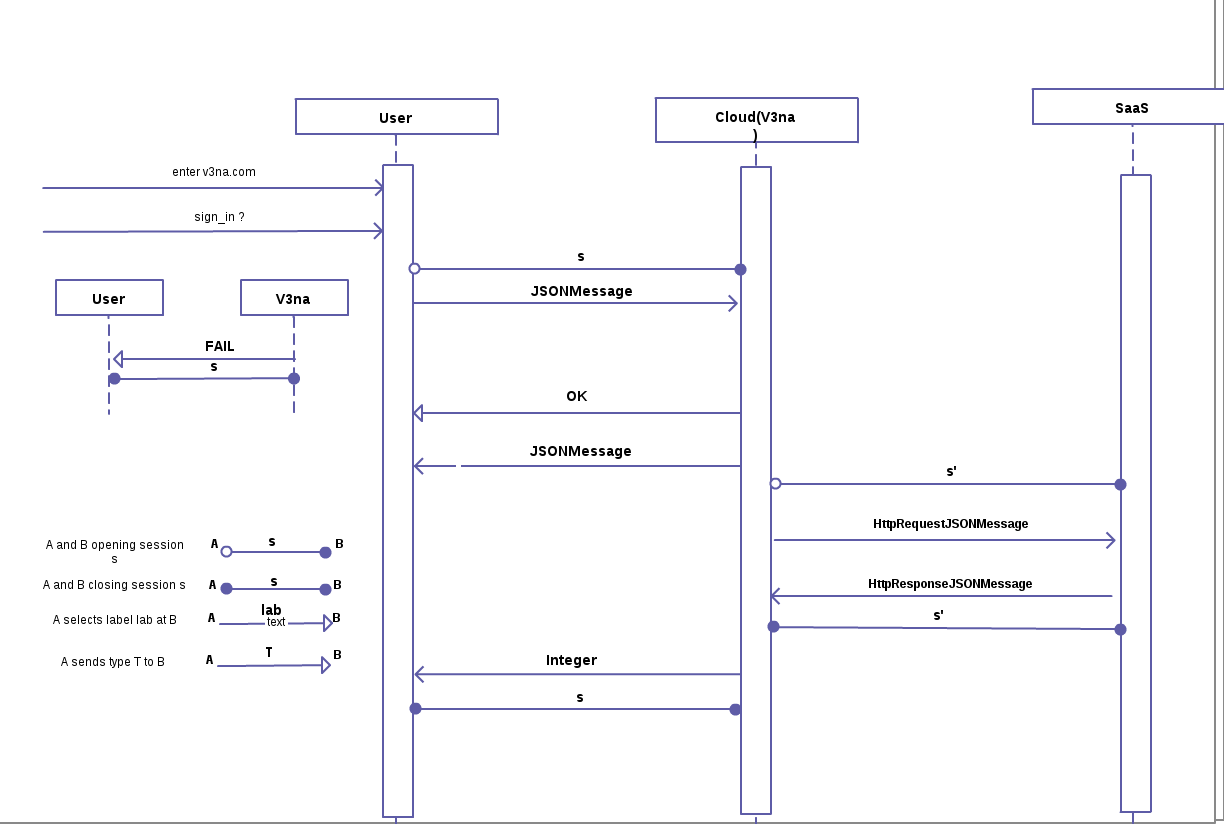
\includegraphics{resources/interaction-sc1.png}}
\caption{Overview of global interactions for Scenario \#1.}
\label{fig:interaction-overview-sc1}
\end{figure}
\end{comment}

%\paragraph{Implementation.}


\subsection{Scenario 2: Session Delegation and Iteration}
%New scenario is a bit harder in complexity.

We present a refined example that demonstrates iteration and session delegation. To avoid becoming a bottleneck, the core processes of the Cloud should delegate the session to a service as soon as the user is authenticated for the service. 

\begin{figure}
\centering
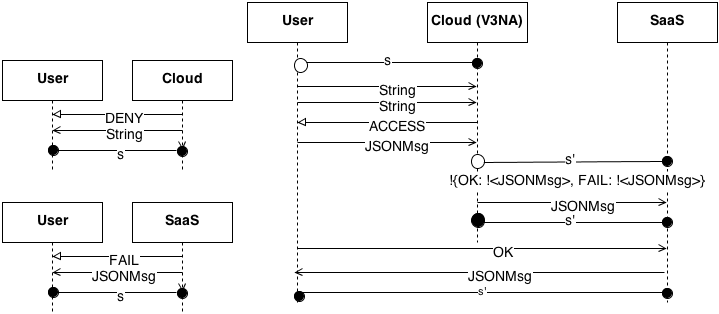
\includegraphics[width=0.8\textwidth]{resources/diag-2.png} %interaction-sc2.png}
\caption{Sequence diagram of interactions for Scenario 2}
\label{fig:seq-diagram-sc2}
\end{figure}

%Figure~\ref{fig:seq-diagram-sc2} describes the global protocol using a sequence diagram.
Figure~\ref{fig:seq-diagram-sc2} depicts two related sessions $s$ and $s'$. Session $s$ begins with interactions between the user and the Cloud; but, after authentication, $s'$ delegates the rest of session $s$ from the Cloud to the service. Session $s$ is completed by an exchange between the user and the service directly.
We informally describe the global protocol in more detail:

\begin{compactenum}
\item  The user begins a request session (session $s$ in Fig.~\ref{fig:seq-diagram-sc2}) with the Cloud (V3na).

\item  The user logs in by providing the Cloud with a user name and password.

\item  V3na receives the user credentials and verifies them: If the user is not authenticated and still has tries %with minimal amount of tries or amount of tries is out of limit,
go back to step 2, otherwise continue.

\item  If the user is not allowed to access the Cloud, the interaction between the user and the Cloud continues on the DENY-branch, otherwise on the ACCESS-branch.

\item  In the case of the ACCESS branch, the user sends his connection request in a JSON message to the Cloud. The Cloud creates a new session with the service (session $s'$ in Fig.~\ref{fig:seq-diagram-sc2}). The new session delegates the remaining session with the user to the service, and also forwards relevant user request details to the service. Session $s'$ is then terminated.

\item  The service continues session $s$, but now interactions are between the user and the service. The service either responds to the user with OK or FAIL. In either case, the user receives the reason and status of his request directly from the service in a JSON message. Finally, session $s$ is terminated.
\end{compactenum}



%\paragraph{Protocols.}
{
\lstset{
  framerule=0pt,
  numbers=none,
  basicstyle=\ttfamily\scriptsize,
}
%\setcounter{lstlisting}{2}
\begin{figure}[h]
\begin{minipage}[t]{0.50\textwidth}
{\it\footnotesize Protocol 2.1: User}
\begin{lstlisting}
protocol p_uv { 
  begin.?[!<String>.!<String> ]*.
  ?{
   ACCESS: !<JSONMsg>.
      ?{
        OK: ?(JSONMsg),
        FAIL: ?(JSONMsg)
      },
   DENY: ?(String)
  } 
}
\end{lstlisting}
\end{minipage}
\begin{minipage}[t]{0.50\textwidth}
{\it\footnotesize Protocol 2.2: Cloud}
\begin{lstlisting}
protocol p_vu { 
  begin.
   ![ ?(String).?(String) ]*. // login
   !{
     ACCESS: ?(JSONMsg).
        !{
          OK: !<JSONMsg>,
          FAIL: !<JSONMsg>
        },
     DENY: !<String>
   } 
}
\end{lstlisting}
\end{minipage}
\caption{User-Cloud interaction protocol specifications for Scenario 2}\label{fig:user-cloud-protocol} 
\end{figure}
}

In Figure~\ref{fig:user-cloud-protocol}, the protocol between the user and the cloud provider appear to interact perfectly. The iterative login step works as expected, so either the ACCESS or DENY branch will be selected. 
If the ACCESS branch is selected, then, as expected, a JSON message is sent from the user to the Cloud. However, instead of the Cloud choosing OK or FAIL directly, the session ($s'$) in Figure~\ref{fig:cloud-saas-providers} is triggered.


%Note that details such as the content of messages and the triggering of one session from another session are at the code level rather than the type level.

%
%The Cloud-Service protocol, Fig.~\ref{fig:cloud-saas-providers}, the session type that is passed as a higher order message is defined separately as protocol $p\_msg$, then referenced using $\mathopen{@}p\_msg$.



%Unlike the previous protocol, the Cloud-Saas protocol significantly altered, also authentication process is added to the protocol in interaction between User --- Cloud.


%\paragraph{Interactions.} The language of the artefacts has already presented in the first scenario.

{
\lstset{
  framerule=0pt,
  numbers=none,
  basicstyle=\ttfamily\scriptsize,
}
\renewcommand\lstlistingname{Protocol}
\setcounter{lstlisting}{0}
\begin{figure}[h]

\begin{minipage}[t]{0.50\textwidth}
{\it\footnotesize Protocol 2.3: Cloud}
\begin{lstlisting}

protocol p_vs {
  begin.
  !<!{
     OK: !<JSONMsg>, 
     FAIL: !<JSONMsg>
  }>.
  !<JSONMsg>    
}

\end{lstlisting}
\end{minipage}
\begin{minipage}[t]{0.50\textwidth}
{\it\footnotesize Protocol 2.4: Service}
\begin{lstlisting}
protocol p_sv {
  begin.
  ?(!{
     OK: !<JSONMsg>,
     FAIL: !<JSONMsg> 
  }).
  ?(JSONMsg) 
}
\end{lstlisting}
\end{minipage}
\caption{Cloud-Service interaction protocol specifications for Scenario 2}\label{fig:cloud-saas-providers} 
\end{figure}
}

The session in Figure~\ref{fig:cloud-saas-providers} delegates the part of the session where either OK or FAIL is selected to the service. 
The delegation is enabled by a higher order session type, where a socket of session type $\mathopen{!}\left\{\texttt{OK}\colon \mathopen{!}\left<\textit{JSONMessage}\right>, \texttt{FAIL}\colon \mathopen{!}\left<\textit{JSONMessage}\right>\right\}$ is sent from the Cloud in protocol $p\_vs$ and received by the service in protocol $p\_sv$. 
%Notice that there is a send $!$ followed by a session type where either OK or FAIL is chosen.
Following, the delegation, a JSON message is sent from the Cloud to the service containing the relevant user request details.


Once the delegation has taken place, the service is able to complete the session that was begun by the Cloud. The service can negotiate directly with the client and either choose the OK branch or the FAIL branch, followed by sending the appropriate JSON message. The simple choice between an OK and a FAIL message could be replaced by a more complex iterated session between the user and the service.

%The $@p$ is syntactically substituted for the protocol of that name.
\begin{comment}
At the implementation level, to receive a higher order message type casting explicitly indicates the received protocol, as in the following code.
\[
\textit{v3na\_user\_socket} = \left(\mathopen{@}\textit{p\_msg}\right)~\textit{v3na\_sv}.\textit{receive}()
\]
The above code defines a socket that receives a session of type $\mathopen{!}\left\{OK\colon \mathopen{!}\left<\textit{JSONMsg}\right>,
FAIL\colon \mathopen{!}\left<\textit{JSONMsg}\right>\right\}$, hence has the type $?\left(\mathopen{!}\left\{OK\colon \mathopen{!}\left<\textit{JSONMsg}\right>,
FAIL\colon \mathopen{!}\left<\textit{JSONMsg}\right>\right\}\right)$.
\end{comment}

\begin{comment}
\paragraph{Implementation.}
Delegating the protocol is straightforward. Simply pass the socket to service using $\textit{s\_vs}.\textit{send}(\textit{user\_vu})$.
To receive a high order message type casting must take place in the case of a protocol, the type of protocol must be explicitly defined, using $\textit{v3na\_user\_socket} = \left(\mathopen{@}\textit{p\_msg}\right)~\textit{v3na\_sv}.\textit{receive}()$, where \textit{p\_msg} is a defined protocol.
Thus we explicitly define the protocol to be delegated and then include it in the final protocol.
\end{comment}

\begin{comment}
\begin{lstlisting}
s_vs.send(user_vu); // pass the remaining protocol
\end{lstlisting}

\begin{lstlisting}
user_vu.outbranch(ACCESS) {
  JSONMessage req_info = user_vu.receive();
  SJServerAddress addr_vs = SJServerAddress.create(p_vs, saas_hname, saas_port);
  SJSocket s_vs = SJRSocket.create(addr_vs); try(s_vs) {
    s_vs.request();
    s_vs.send(user_vu); // pass the remaining protocol    
    s_vs.send(req_info);
  } catch(UnknownHostException uhe) {
    uhe.printStackTrace(); 
  }
}
\end{lstlisting}
\end{comment}
\begin{comment}
\begin{lstlisting}
v3na_user_socket = (@p_msg) v3na_sv.receive();
\end{lstlisting}
\end{comment}


%------------------------------------------------------------------------------


\section{Future Work: Inter-Cloud Protocols and Session Types}
\label{sect:highlights}

For customers of Cloud providers, there are considerable benefits when service can be hosted on more than one Cloud provider~\cite{Buyya2009,intercloud,Armbrust2010}.
If data is replicated across multiple Cloud providers, customers can avoid becoming locked in to one provider. Thus customers are less exposed to risks such as fluctuations in prices and quality of service at a single provider. If a Cloud provider goes out of business, then customers entirely dependent on one Cloud provider are critically exposed.
%If data is replicated across multiple services providers, we 
%Benefits include geographic replication for highly available robust services, and a greater ability to circumvent legal and technical restrictions. 
%is moving to the concept where Cloud operated by one enterprise interoperating with a Cloud of another is powerful idea.
%So far that is limited to use cases where code running on one cloud explicitly references a service on another cloud.
%For improved interoperability, inter-Cloud protocols are prosed as future standards. %this we require protocols There is no implicit and transparent interoperability. 

Several visions have been proposed for inter-Cloud protocols~\cite{xmpp-intercloud-transport,cloud-integrator}. In~\cite{utility-driven-fed}, they identify the main components of general inter-Cloud architecture:
%\begin{inparaenum}[(\bgroup\bfseries a\egroup)]
%\item
a \textit{Cloud coordinator}, for exposing Cloud services;
%\item
a \textit{Cloud broker}, for mediating between service consumers and Cloud coordinators;
%\item
and a \textit{Cloud exchange}, for collecting consumers' demands and locating Cloud providers. % with them with offers.
%\end{inparaenum}
%
Based on our experience in this work, we suggest that multi-party session types~\cite{ng2012multiparty} are appropriate for specifying and correctly implementing protocols between Cloud providers and Cloud integrators.

%Implementations of protocols should be extended at the socket layer, so that the protocols are monitored at runtime to check that interactions conform to a protocol verified using session types.
%Session types can reduce the potential risks of using protocols where each participant is developed and hosted by competing businesses.
%Each processes for each role (either Cloud provider or Cloud Exchange) can then be implemented are implemented in Erlang or Python (they are best for working with high load applications).
%Since all the roles should be aware of each other in global network in order to dialog with each other, we
%We propose using SockJS\footnote{SockJS is an effort to define a protocol between in-browser SockJS-client and its server-side counterparts} protocol for presence and AMQP messaging (it's thin, flexible).
%We specify the interactions of an inter-Cloud protocol.
%Since the  and, as a result, the whole communication is safe.
%As a starting point for dynamic verification observers, we referred to \cite{safe-conver-prog-python} work.
%Session-based programming has been applied in various fields, including parallel algorithms~\cite{sj-parallel}, event-driven programming~\cite{event-driven-sj} and multi-party conversations~\cite{sj-business-protocols}.


\section{Conclusion}
\label{sect:conclusion}
This case study demonstrates the ability of session types to control interaction patterns between communicating processes in a Cloud.
Participants are statically type-checked at compile time and dynamically monitored at run-time to ensure that components critical to a Cloud provider communicate correctly.
The high level of abstraction of session types, implemented in the SessionJ language, enabled effortless translation of business scenarios into protocols.
We were able to refine our protocol from Scenario 1 to Scenario 2, due to support of higher-order message passing (session delegation). %, allowed us to refine from Scenario 1 to Scenario 2.
Further to scenarios presented here, our case study covered payment and wallet recharging transactions, %(available by \url{https://github.com/Rustem/Master-thesis}),
where we discovered the benefits of combining session delegation and threading provided by SessionJ.
Our experience shows that the session-programming approach is suited to correctly implementing inter-Cloud protocols, which is our future objective. %Finally, hope that our feedback about session types will be as a solid starting point for further research in this area.  

\paragraph{Acknowlegements.} We thank the anonymous reviewers for their clear and constructive comments. We are grateful to Ramesh Kini for his support for this project.


%------------------------------------------------------------------------------
% Refs:
%
\label{sect:bib}
\bibliographystyle{plain}
%\bibliographystyle{alpha}
%\bibliographystyle{unsrt}
%\bibliographystyle{abbrv}
\bibliography{easychair}

%------------------------------------------------------------------------------
\appendix



%------------------------------------------------------------------------------
% Index
%\printindex

%------------------------------------------------------------------------------
\end{document}

% EOF
